\begin{frame}\frametitle{Bugs tracking and community of simgrid}
There are few several ways that we use to support the community, improve continuously simgrid, and interact with the other members.
\begin{enumerate}
\item Follow the mailing lists to be aware about the issues that face the community \textcolor{blue}{\url{simgrid-user@lists.gforge.inria.fr}}. 
\item Participate in discussions on \textcolor{blue}{IRC} channel \textcolor{blue}{$\# $simgrid} on \textcolor{blue}{oftc} servers. %The channel allowed to having exchange of ideas, resolve issues efficiently and having back up if one is in trouble. 
\item Attend scheduled meetings by project members to get an idea of the different parts of the code.
\item Participate to the bug tracking via \textcolor{blue}{Github issues} and \textcolor{blue}{Sonar}.
\end{enumerate}
\end{frame}
\begin{frame}\frametitle{Workflow}
\begin{figure}
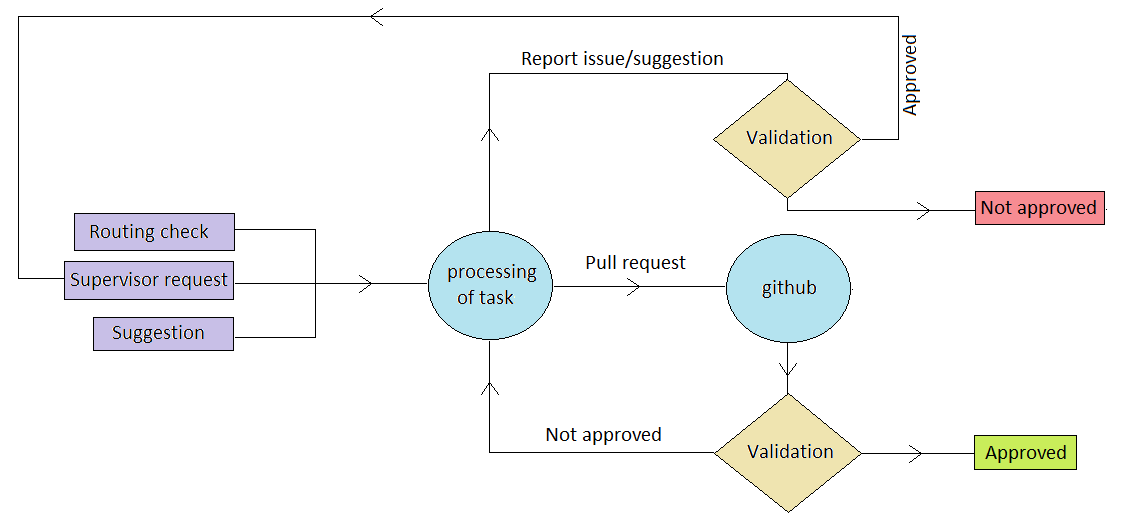
\includegraphics[width=11cm]{figures/productiont.png}
\end{figure}
\end{frame}
\begin{frame}\frametitle{Validation tools}
SimGrid dispose of a bunch of testing procedures that are used to detect bugs and bad written of code.
\begin{itemize}
\item \textcolor{blue}{Jenkins} : a self-contained automation server which allowed to automate any kind of tasks related to building, testing, and deploying software.
\item \textcolor{blue}{Travis-ci} : a hosted, distributed continuous integration service used to build and test software projects hosted at GitHub.
\item \textcolor{blue}{Codacy} : an automated code review application that includes static analysis functionality.
\item \textcolor{blue}{SonarQube} : an open source platform for inspect the code quality with static analysis of code.
\end{itemize}

\end{frame}